%%% ------------------------------------------------------------------
%%% Laboratory 1 -- Short project
%%% Cloud computing
%%% Master's degree in Machine Learning and Cybersecurity
%%% for Internet Connected Systems -- UPC (EPSEM)
%%%
%%% Build:   make          Clean:  make clean
%%%
%%% One file per section in sections/. Each team member edits only the
%%% sections they own (README.md). \todo{...} prints pending
%%% work in red: the delivered PDF must contain none.
%%% ------------------------------------------------------------------

\documentclass[informe,english]{practicaitic}
\usepackage{mlcsreport}
\usepackage{lst-shell}
\usetikzlibrary{fit,backgrounds}

%% Keep "--" as two hyphens in typewriter text, for command options.
\DisableLigatures[-]{encoding = *, family = tt*}

%% The statement calls it "Laboratory 1: Short project".
\renewcommand{\reportkind}{Laboratory}

%% Pending work, printed in red so nothing is forgotten.
\newcommand{\todo}[1]{\textcolor{upcred}{\textbf{[TODO:}~#1\textbf{]}}}

\numpract{1}
\course{Cloud computing}
\titol{Short project --- a microservices infrastructure on Docker Swarm}
\autor{Víctor Martín Castilla\and Mikael Rodriguez\and Bernat Ventura}

\begin{document}

\begin{abstract}
  The team containerised a company's services as four Docker stacks on a
  Swarm of three Azure virtual machines that share an NFS disk: shared
  basic services, a ratings-monitor application, a Moodle learning
  platform, and monitoring with Prometheus and Grafana. One node is the
  only public entry: nginx ends HTTPS with a Let's Encrypt certificate and
  routes each address to its stack. Every stack has a local Compose file
  and a production file, and the team builds its images and keeps them in
  its own registry. On 19 October all 18 services ran with their full
  replica count. Stateless services run two replicas and update one at a
  time with automatic rollback, and both databases have a verified daily
  backup.
  The main result is that data outlives containers: the app's database
  moved between nodes with its data intact, and a restore drill brought
  a deleted Moodle course back in 21~seconds. The main gap is that the
  backups still share a disk with the data they protect.
\end{abstract}

%% Owner: Víctor Martín Castilla
\section{Introduction}
\label{sec:introduction}

The short project asks for the digital transformation of a company's
infrastructure into containerised microservices
\parencite{llusa2026project}. The company runs four groups of services,
each deployed as its own Docker stack: shared basic services, a core
application, an observability platform and a Moodle learning management
system. Everything must run on a Docker Swarm of at least three nodes,
be described by Compose files, and scale to several containers, except
for cron jobs and database engines that cannot.

Deploying may only take two kinds of step: building images and deploying
the Compose files. Two Compose files are required per stack: one for a
local environment without TLS or mapped volumes, and one with the full
production configuration.

The team has three members rather than the five the statement assumes,
so the work was split by stack, with one owner per stack and every
change reviewed through a pull request (\cref{sec:team}).

\Cref{sec:architecture} describes the services and how they map to
stacks. \Cref{sec:infrastructure} explains where the cluster runs and how
its virtual machines were created and secured, and \cref{sec:swarm} how
the Swarm was built on them. Sections~\ref{sec:stack-basic}
to~\ref{sec:stack-stats} cover each stack, \cref{sec:data} the data and
its backups, \cref{sec:hadr} high availability and disaster recovery, and
\cref{sec:deployment} the deployment procedure.

%% Owner: Víctor Martín Castilla
\section{Architecture}
\label{sec:architecture}

The statement fixes the services and groups them into stacks
\parencite{llusa2026project}. Each stack is one Compose file deployed as
one Swarm stack, so it can be developed, deployed and rolled back on its
own \parencite{llusa2026compose,llusa2026orchestration}.

\begin{description}
  \item[basic] Shared services. An nginx front proxy receives all public
    traffic and forwards it to the other stacks. Certbot obtains and
    renews Let's Encrypt certificates for it. A private registry stores
    the images the team builds, and an NFS export provides the disk
    shared between nodes.
  \item[app] The company's core application, a Python web service, with
    its PostgreSQL database, a Redis cache, an Apache server for static
    files, an SMTP relay towards an external mail provider, an automatic
    feeder that captures ratings and posts them to the application, and a
    cron job that dumps the database. \todo{describe what the core app
    does once it exists.}
  \item[atenea] The Moodle learning management system with its MariaDB
    database, the Moodle cron and a backup job.
  \item[stats] Grafana, provisioned from files following the
    observability-as-code approach, with Prometheus as its metrics store,
    node exporter and cAdvisor on every node, and a Grafana plugin.
    \todo{name the plugin and justify the choice.}
\end{description}

\Cref{tab:services} lists every service with its number of replicas and
where Swarm may place it. The statement requires every service to scale
to several containers, except cron jobs and database engines that do not
allow it \parencite{llusa2026project}. Every single-replica row falls in
one of those two groups. Prometheus counts as a database because it keeps
its time series on local disk. Redis counts as one because two
independent instances behind one virtual IP would hold two different
caches.

\begin{table}[htbp]
  \centering
  \caption{Services, replicas and placement. ``Any'' means Swarm chooses
    the node; \texttt{role=\ldots} pins the service to the node carrying
    that label (\cref{sec:swarm}).}
  \label{tab:services}
  \small
  \begin{tabular}{lllll}
    \toprule
    Stack  & Service          & Replicas  & Placement                    & Reason \\
    \midrule
    basic  & nginx front      & 2 or more & any                          & stateless \\
           & certbot          & 1         & \texttt{role=entry}          & cron job \\
           & registry         & 2         & any, storage on NFS          & shared storage \\
           & off-site copy    & 1         & \texttt{role=entry}          & cron job \\
    \midrule
    app    & core app         & 2 or more & any                          & stateless \\
           & PostgreSQL       & 1         & \texttt{role=db}             & DBMS \\
           & Redis            & 1         & any                          & DBMS, cache only \\
           & static Apache    & 2 or more & any                          & stateless \\
           & SMTP relay       & 2         & any                          & stateless \\
           & auto feeder      & 2         & any                          & stateless \\
           & database dump    & 1         & any                          & cron job \\
    \midrule
    atenea & Moodle           & 2 or more & any, files on NFS            & shared storage \\
           & MariaDB          & 1         & \texttt{role=db}             & DBMS \\
           & Moodle cron      & 1         & any                          & cron job \\
           & Moodle backup    & 1         & any                          & cron job \\
    \midrule
    stats  & Grafana          & 2         & any                          & shared database \\
           & Grafana database & 1         & \texttt{role=monitoring}     & DBMS \\
           & Prometheus       & 1         & \texttt{role=monitoring}     & time-series DBMS \\
           & node exporter    & global    & every node                   & one per host \\
           & cAdvisor         & global    & every node                   & one per host \\
    \bottomrule
  \end{tabular}
\end{table}

One component is not a container. The NFS server runs on the host
system of one node, because a kernel NFS server needs privileged mode,
which Swarm services do not support.

%% Owner: Víctor Martín Castilla
\section{Infrastructure}
\label{sec:infrastructure}

\todo{Rewrite for the cluster the team uses: three Azure VMs built by
Mikael. Document where they run, meaning subscription type, region, VM
size and operating system. Document the network: address space, which
VMs have public IPs, and the firewall rules. Then how the VMs were
created and prepared, ideally as code; access control and SSH
hardening, with evidence; the options the team considered for hosting;
and the cost. Text about an earlier cluster, built and deleted on
17 October, is in the git history if anything is worth reusing.}

\subsection{Requirements}
\label{sec:infra-requirements}

The statement asks for a Swarm of at least three nodes and leaves the
hosting open: home hardware, virtual machines on a laptop, or a public
cloud \parencite{llusa2026project}. The choice had to meet five
constraints:
\begin{itemize}
  \item three machines that stay on, so the cluster works whenever it is
        checked;
  \item a public address for the front proxy, so Let's Encrypt can
        validate the domain and users can reach the services;
  \item a private network between the nodes for Swarm and NFS traffic;
  \item no cost for the team;
  \item ready within the two days left before the deadline.
\end{itemize}

\subsection{Why three nodes}
\label{sec:infra-three}

Swarm managers keep the cluster state with the Raft consensus algorithm
\parencite{ongaro2014raft,llusa2026orchestration}. A change is committed
only when a majority of managers agree, so a cluster of $N$ managers
survives $\lfloor (N-1)/2 \rfloor$ manager failures
\parencite{docker-raft}. \Cref{tab:raft} shows why two managers are no
better than one, and why three is the smallest cluster that survives a
failure. All three nodes should therefore be managers, and they also run
workloads.

\begin{table}[htbp]
  \centering
  \caption{Manager failures a Swarm survives while keeping a majority.}
  \label{tab:raft}
  \begin{tabular}{ccc}
    \toprule
    Managers & Majority & Failures survived \\
    \midrule
    1 & 1 & 0 \\
    2 & 2 & 0 \\
    3 & 2 & 1 \\
    5 & 3 & 2 \\
    \bottomrule
  \end{tabular}
\end{table}

%% Owner: Víctor Martín Castilla
\section{Swarm cluster}
\label{sec:swarm}

All three nodes are Swarm managers, so the cluster keeps working when one
of them fails (\cref{sec:infra-three}). Each node advertises its private
address, so Swarm traffic never leaves the subnet. \Cref{tab:nodes} shows
the nodes as the security review of 17 October found them.

\begin{table}[htbp]
  \centering
  \caption{The Swarm's nodes, as \texttt{docker node ls} reports them.}
  \label{tab:nodes}
  \begin{tabular}{lll}
    \toprule
    Node                     & Status & Manager status \\
    \midrule
    \texttt{swarm-manager-1} & Ready  & Reachable \\
    \texttt{swarm-manager-2} & Ready  & Leader \\
    \texttt{swarm-manager-3} & Ready  & Reachable \\
    \bottomrule
  \end{tabular}
\end{table}

\subsection{Placement}

Pinned services name their node in a placement constraint on its host
name. nginx, for example, runs where
\texttt{node.hostname == swarm-manager-1}. Node labels would read
better, but each one is a manual command on the cluster, while host names
need no step beyond deploying the Compose file.

\subsection{Networks}

Every stack has its own overlay network for internal traffic, such as a
database and its clients. A shared overlay network, \texttt{proxy},
connects nginx with the public services of every stack, which join it
under an alias such as \texttt{app-core} or \texttt{atenea-moodle}. nginx
resolves these names through Docker's DNS on every request, so it starts
even when a stack is missing. \texttt{proxy} is created once, outside any
stack, so that every stack can declare it as external.

nginx publishes ports 80 and 443 through the routing mesh, so every node
listens on them. The security groups only let that traffic reach
\texttt{swarm-manager-1}.

\subsection{Shared disk}

\texttt{swarm-manager-1} runs the kernel NFS server and exports
\texttt{/srv/nfs} to the subnet only. The other two nodes mount it with
NFS~4.2 at the same path, from \texttt{/etc/fstab}, so a bind mount of a
folder under \texttt{/srv/nfs} gives the same files on every node. Swarm
refuses a bind mount whose source does not exist, so a service that
needs a new folder mounts the whole share and creates the folder itself.

The export first squashed root, mapping it to \texttt{nobody} on the
client nodes. The registry, on \texttt{swarm-manager-2}, could not store
images, so the export switched to \texttt{no\_root\_squash}, still
restricted to \texttt{10.0.1.0/24}. The price is that root in any
container that mounts the share acts as root on every shared file.
Services that face the internet should therefore mount only their own
folder, as the Moodle replicas do (\cref{sec:stack-atenea}).

\subsection{Validation}

\begin{itemize}
  \item \textbf{Firewall.} From the internet, only
        \texttt{swarm-manager-1} answers, on ports 22, 80 and 443
        (\cref{sec:infra-network}).
  \item \textbf{Shared disk.} During a redeploy, Swarm moved the app's
        PostgreSQL from \texttt{swarm-manager-1} to
        \texttt{swarm-manager-3}, and the new server found its data
        (\cref{sec:app-nfs}).
  \item \textbf{Overlay network and routing mesh.} The app answers at its
        subdomain through nginx on \texttt{swarm-manager-1}, while its
        replicas run spread over the three nodes (\cref{sec:stack-app}).
\end{itemize}

%% Owner: Mikael Rodriguez
\section{Stack: basic}
\label{sec:stack-basic}

\todo{Owner: Mikael Rodriguez. Cover, in this order:
the services and the image each one uses;
the Dockerfiles you wrote and why;
the differences between \texttt{compose.yml} and \texttt{production.yml};
replicas, placement and update policy;
volumes, NFS paths and secrets;
health checks and metrics;
how you tested it locally and on the Swarm.}

%% Owner: Bernat Ventura
\section{Stack: app}
\label{sec:stack-app}

The app stack is a ratings monitor. The statement suggests, as the
automatic feeder, ``a monitor that captures comment ratings on web
pages'' \parencite{llusa2026project}, and the whole application is
built around that idea, so every service has a real job. Many web pages
publish their rating as schema.org JSON-LD (\texttt{aggregateRating}),
the format search engines read to show stars. The feeder reads that
rating from a list of pages, the core application stores it and shows
the latest rating of each page at
\url{https://app.ccds-project.duckdns.org}, and it can email the
summary as a report. The pages are two books on Goodreads, two recipes
on BBC Good Food and a film on Rotten Tomatoes. Other sites, such as
IMDb or Allrecipes, were tested and dropped because they do not publish
the rating in that format.

\subsection{Services and images}

\Cref{tab:app-services} lists the seven services. Five images are built
by the team and pushed to the registry of the basic stack as
\texttt{ccds-project.duckdns.org/app-<service>:<version>}; Redis uses the
official image unchanged.

\begin{table}[htbp]
  \centering
  \caption{Services of the app stack.}
  \label{tab:app-services}
  \small
  \begin{tabular}{llll}
    \toprule
    Service & Image                         & Replicas & Role \\
    \midrule
    core    & \texttt{app-core} (Flask)     & 2 & web page and API \\
    static  & \texttt{app-static} (httpd)   & 2 & static files under \texttt{/static/} \\
    db      & \texttt{app-db} (PostgreSQL 17) & 1 & ratings, data on NFS \\
    redis   & \texttt{redis:8.2-alpine}     & 1 & 30\,s cache of the summary \\
    smtp    & \texttt{app-smtp} (msmtpd)    & 2 & relays mail to Gmail on port 587 \\
    backup  & \texttt{app-backup} (crond)   & 1 & nightly \texttt{pg\_dump} to NFS \\
    auto    & \texttt{app-auto} (Python)    & 2 & reads the ratings, posts them to core \\
    \bottomrule
  \end{tabular}
\end{table}

A rating flows through the stack as follows. Each \texttt{auto} replica
downloads its pages, extracts the \texttt{aggregateRating} with a
regular expression and a search of the JSON tree, and posts it to
\texttt{core} with a shared token. \texttt{core} inserts it into one
PostgreSQL table. The summary is a single
\texttt{SELECT DISTINCT ON (url)} that keeps the latest rating of each
page. It follows the cache-aside pattern: \texttt{core} first asks
Redis, and on a miss queries PostgreSQL and stores the result for
30\,seconds. If Redis is down, the page still works from the database.
\texttt{POST /api/report} sends the summary by email through
\texttt{smtp}.

\subsection{Dockerfiles}

\begin{description}
  \item[core and auto] \texttt{python:3.13-slim}, pinned dependencies,
    and an unprivileged user. \texttt{core} runs gunicorn with one
    worker and eight threads: the stack scales by adding replicas, not
    workers inside a container.
  \item[static] \texttt{httpd:2.4-alpine} with the files copied under
    \texttt{htdocs/static/}, because nginx forwards the path unchanged,
    plus cache headers.
  \item[db] The official PostgreSQL image with a small entrypoint in
    front. It creates the data directory on NFS, owned by
    \texttt{postgres} (uid 70), and then runs the official entrypoint
    as \texttt{postgres}. \Cref{sec:app-nfs} explains why.
  \item[smtp] \texttt{alpine:3.22} with \texttt{msmtpd}, a minimal SMTP
    server that hands every message to \texttt{msmtp}, which relays it
    to the provider with authentication and STARTTLS. Azure blocks
    outbound port 25 \parencite{azure-smtp}, so the relay uses port 587.
  \item[backup] The same PostgreSQL image, so \texttt{pg\_dump} matches
    the server version, with busybox \texttt{crond}.
\end{description}

\subsection{Local and production files}

\texttt{compose.yml} runs the stack on a laptop with
\texttt{docker compose up}. It is self-contained: it adds its own nginx
on port 8080 in place of the basic stack, replaces the relay with
Mailpit, which catches every email and shows it on port 8025, keeps the
data in named volumes, passes passwords as plain environment variables,
and feeds two demo pages served by \texttt{static}, so it works without
internet access. \texttt{production.yml} is the Swarm version: images
from the registry, data on NFS, Swarm secrets, the external
\texttt{proxy} network shared with nginx, replicas and update policies.

\subsection{Replicas, placement and updates}

The four stateless services run two replicas each, and Swarm may place
them on any node. Three services run one replica, all within the
exceptions of the statement \parencite{llusa2026project}:
\texttt{db} is a DBMS, \texttt{backup} is a cron job, and \texttt{redis}
is an in-memory database used as a shared cache, since two independent
instances behind one virtual IP would hold two different caches.

The feeder replicas share the work without talking to each other. Swarm
gives every task a slot number, \texttt{\{\{.Task.Slot\}\}}, passed as
\texttt{FEEDER\_SLOT}. With $N$ replicas, replica $k$ takes URLs
$k, k+N, k+2N, \ldots$ (\texttt{URLS[SLOT-1::REPLICAS]} in Python), so
each page is read by exactly one replica.

Stateless services update one task at a time, start the new task before
stopping the old one, and roll back if the update fails. The database
uses \texttt{stop-first} instead, because two PostgreSQL servers must
never open the same data directory.

\subsection{Data, NFS and secrets}
\label{sec:app-nfs}

PostgreSQL keeps its data in \texttt{/srv/nfs/app/db} and the dumps go
to \texttt{/srv/nfs/app/backups}, both on the NFS share that every node
mounts. Swarm refuses a bind mount whose source directory does not
exist, so \texttt{db} and \texttt{backup} mount the whole share and
create their own directory on start. This only works if root in a
container can write to the share. The export first used
\texttt{root\_squash}, which maps root to \texttt{nobody} on the client
nodes. That broke the registry, which ran on manager-2 and could not
store new images, and it would have broken the database too. The export
now uses \texttt{no\_root\_squash}, restricted to the cluster subnet
\texttt{10.0.1.0/24}.

The data really is shared. During a redeploy Swarm stopped PostgreSQL on
manager-1 and started it on manager-3, and the new server found the
data where the old one had left it.

Three values are Swarm secrets: the database password, the token that
protects the write endpoints, and the SMTP password, which is a Gmail
app password of an account created for the project. Their files live
only on the deploying node, in \texttt{app/secrets/}, which git ignores
because the repository is public. Secrets cannot change in place, so
each name carries a version (\texttt{app\_smtp\_password\_v2}) that is
raised when the file changes.

The dumps are described with the other databases in \cref{sec:data}:
\texttt{pg\_dump} in custom format every night at 03:00, a check with
\texttt{pg\_restore --list} before a dump is kept, and seven days of
retention. Redis holds nothing worth a backup.

\subsection{Health checks and metrics}

\texttt{core} answers \texttt{/healthz} and \texttt{static} serves its
stylesheet; both are image health checks, so Swarm replaces a task that
stops answering. The \texttt{smtp} check only tests that \texttt{msmtpd}
runs: opening an SMTP session every 30\,seconds filled the logs with
aborted sessions. \texttt{core} exposes Prometheus metrics at
\texttt{/metrics}: cache hits and misses, and ratings received. nginx
answers 404 to that path from outside. Prometheus does not scrape it:
the stats stack only scrapes node exporter and cAdvisor.

\subsection{Testing}

Locally, \texttt{docker compose up --build} built the five images, the
feeder read both demo pages, \texttt{/api/pages} returned their
ratings, and the report email appeared in Mailpit. The first local run
failed with a 502: the local nginx had resolved \texttt{core} when it
started and kept the old address after \texttt{core} was recreated. It
now resolves the name on every request, as the nginx of the basic stack
does.

On the Swarm, all seven services reached their replica count across the
three nodes. The public endpoint returns the five pages, and a report
reached a real mailbox through Gmail. Two problems appeared on the
way: the registry could not store images because of
\texttt{root\_squash}, and the first SMTP attempt failed because the
user name was still the example value; the relay log showed Gmail's
answer, \texttt{535 Username and Password not accepted}.

%% Owner: Víctor Martín Castilla
\section{Stack: atenea}
\label{sec:stack-atenea}

\todo{Owner: Víctor Martín Castilla. Cover, in this order:
the services and the image each one uses;
the Dockerfiles you wrote and why;
the differences between \texttt{compose.yml} and \texttt{production.yml};
replicas, placement and update policy;
volumes, NFS paths and secrets;
health checks and metrics;
how you tested it locally and on the Swarm.}

%% Owner: Mikael Rodriguez
\section{Stack: stats}
\label{sec:stats}
The stats stack provides monitoring for the Docker Swarm cluster.
Prometheus collects and stores metrics, while Grafana displays them
in dashboards. Node Exporter collects host metrics and cAdvisor
collects container metrics. This allows us to monitor resource usage
and check that metrics are available across the cluster.

\subsection{Services and images}
The stack uses four services, listed in \Cref{tab:services}.
\begin{table}[htbp]
\centering
\caption{Services of the stats stack.}
\label{tab:services}
\small
\begin{tabular}{l>{\raggedright\arraybackslash}p{48mm}>{\raggedright\arraybackslash}p{60mm}}
\toprule
Service & Image & Role \\
\midrule
Prometheus & Official Prometheus image
& Scrapes and stores metrics from the exporters \\
Grafana & Custom Grafana image
& Displays metrics in dashboards and includes the required
datasource plugin \\
Node Exporter & Official Prometheus Node Exporter image
& Exposes CPU, memory, disk and network metrics from
the host \\
cAdvisor & Official cAdvisor image
& Exposes resource usage metrics for Docker containers \\
\bottomrule
\end{tabular}
\end{table}

Prometheus scrapes Node Exporter on port 9100 and cAdvisor on port
8080. Grafana uses the Prometheus datasource at
\texttt{http://prometheus:9090} to query the collected metrics.

\subsection{Dockerfiles}
Only Grafana requires a custom Dockerfile. It extends the official
Grafana image and installs the plugin needed by the project. Building
this image ensures that the plugin is available whenever the service
starts, without having to install it manually through the Grafana
interface.

The other services use official images. Their configuration is supplied
through the Compose files and Prometheus configuration.

After changing the Dockerfile or plugin version, the Grafana image
must be rebuilt and published to the registry before deploying the
updated image to the Swarm.

\subsection{\texttt{compose.yml} and \texttt{production.yml}}
The local Compose file is used to test monitoring on a developer
machine, while \texttt{production.yml} deploys the services on Swarm.
The main differences are shown in \Cref{tab:diff}.
\begin{table}[htbp]
\centering
\caption{Differences between local and production monitoring.}
\label{tab:diff}
\small
\begin{tabular}{>{\raggedright\arraybackslash}p{28mm}>{\raggedright\arraybackslash}p{49mm}>{\raggedright\arraybackslash}p{51mm}}
\toprule
& \texttt{compose.yml} & \texttt{production.yml} \\
\midrule
Deployment & Local Docker Compose
& Docker Swarm stack \\
Images & Local or published images
& Published images available to Swarm nodes \\
Discovery & Compose service names
& Docker DNS discovery of Swarm tasks \\
Networking & Compose network
& Overlay network \texttt{monitoring\_backend} \\
Configuration & Local files and mounts
& Swarm configs and production settings \\
Placement & Local machine
& Services placed according to Swarm constraints \\
Storage & Local volumes
& Production volumes or host paths, as configured \\
\bottomrule
\end{tabular}
\end{table}

In production, Prometheus discovers exporter tasks through DNS:
\texttt{tasks.monitoring\_node-exporter} and
\texttt{tasks.monitoring\_cadvisor}. This avoids maintaining a static
list of task IP addresses and allows Prometheus to discover tasks as
they change.

\subsection{Replicas, placement and update policy}
Each monitoring service runs one replica. Prometheus and Grafana are
placed on \texttt{swarm-manager-1}, which provides a predictable
location for the central monitoring services. This also aligns with
the node used to access Grafana through the nginx reverse proxy.

Placement constraints and local storage requirements must be
considered when rescheduling these services.

Node Exporter and cAdvisor run on the Swarm nodes to expose host and
container metrics. Prometheus discovers their tasks through the
\texttt{monitoring\_backend} overlay network.

With one replica, restarting or updating Prometheus or Grafana can
temporarily interrupt monitoring. Updates must use the image and
configuration versions defined in the production stack file.

\subsection{Volumes, NFS paths and secrets}
Prometheus needs persistent storage if collected time-series data
must survive container replacement. Grafana may also use persistent
storage for data maintained inside Grafana. The exact volume mounts
are defined in the stack configuration.

The \texttt{monitoring\_backend} overlay network allows Prometheus
to reach the exporters and Grafana to reach Prometheus by service
name. Node Exporter and cAdvisor also expose ports 9100 and 8080
in the configured deployment, but their metrics should not be
published publicly without a reason.

Grafana's administrator password must be configured securely rather
than committed to the repository. For local testing, create a password
in an environment file excluded from Git, or supply it through the
local environment. In production, use the secret or environment
mechanism defined by the deployment configuration. Do not put real
passwords in the Compose files or documentation.

For example, generate a strong password locally with:
\begin{shell}
openssl rand -base64 24
\end{shell}

Store the generated value in the appropriate local environment file
or production secret. Restrict access to the file and ensure it is
excluded from version control. If the configuration uses a Swarm
secret, create it before deploying the stack and reference its
actual name in \texttt{production.yml}.

\subsection{Health checks and metrics}
Prometheus scrapes the exporters every 15 seconds. Node Exporter
provides host-level metrics, while cAdvisor provides container-level
metrics. Grafana uses these measurements to display CPU, memory,
disk, network and container usage.

The Prometheus Targets page shows whether each exporter is being
scraped successfully. Grafana dashboards provide a visual overview
of the collected metrics. These checks are separate from Docker
health checks: a running container does not necessarily mean that
Prometheus can scrape its metrics.

\subsection{Testing}
\paragraph{Locally.}
Start the local monitoring stack and check the containers:
\begin{shell}
docker compose -f stats/compose.yml up -d
docker compose -f stats/compose.yml ps
docker compose -f stats/compose.yml logs prometheus
\end{shell}

Open Grafana at the address and port configured in
\texttt{compose.yml}. Log in using the local administrator credentials.
Check that the Prometheus datasource is working, then open the
Prometheus Targets page and confirm that the configured targets are
healthy.

If the local configuration publishes Prometheus on port 9090, its
targets page can be opened at:
\begin{shell}
http://localhost:9090/targets
\end{shell}

Check that the dashboards display data rather than empty graphs.
The local dashboard is shown in \Cref{fig:local-dashboard}.
\begin{figure}[htbp]
\centering
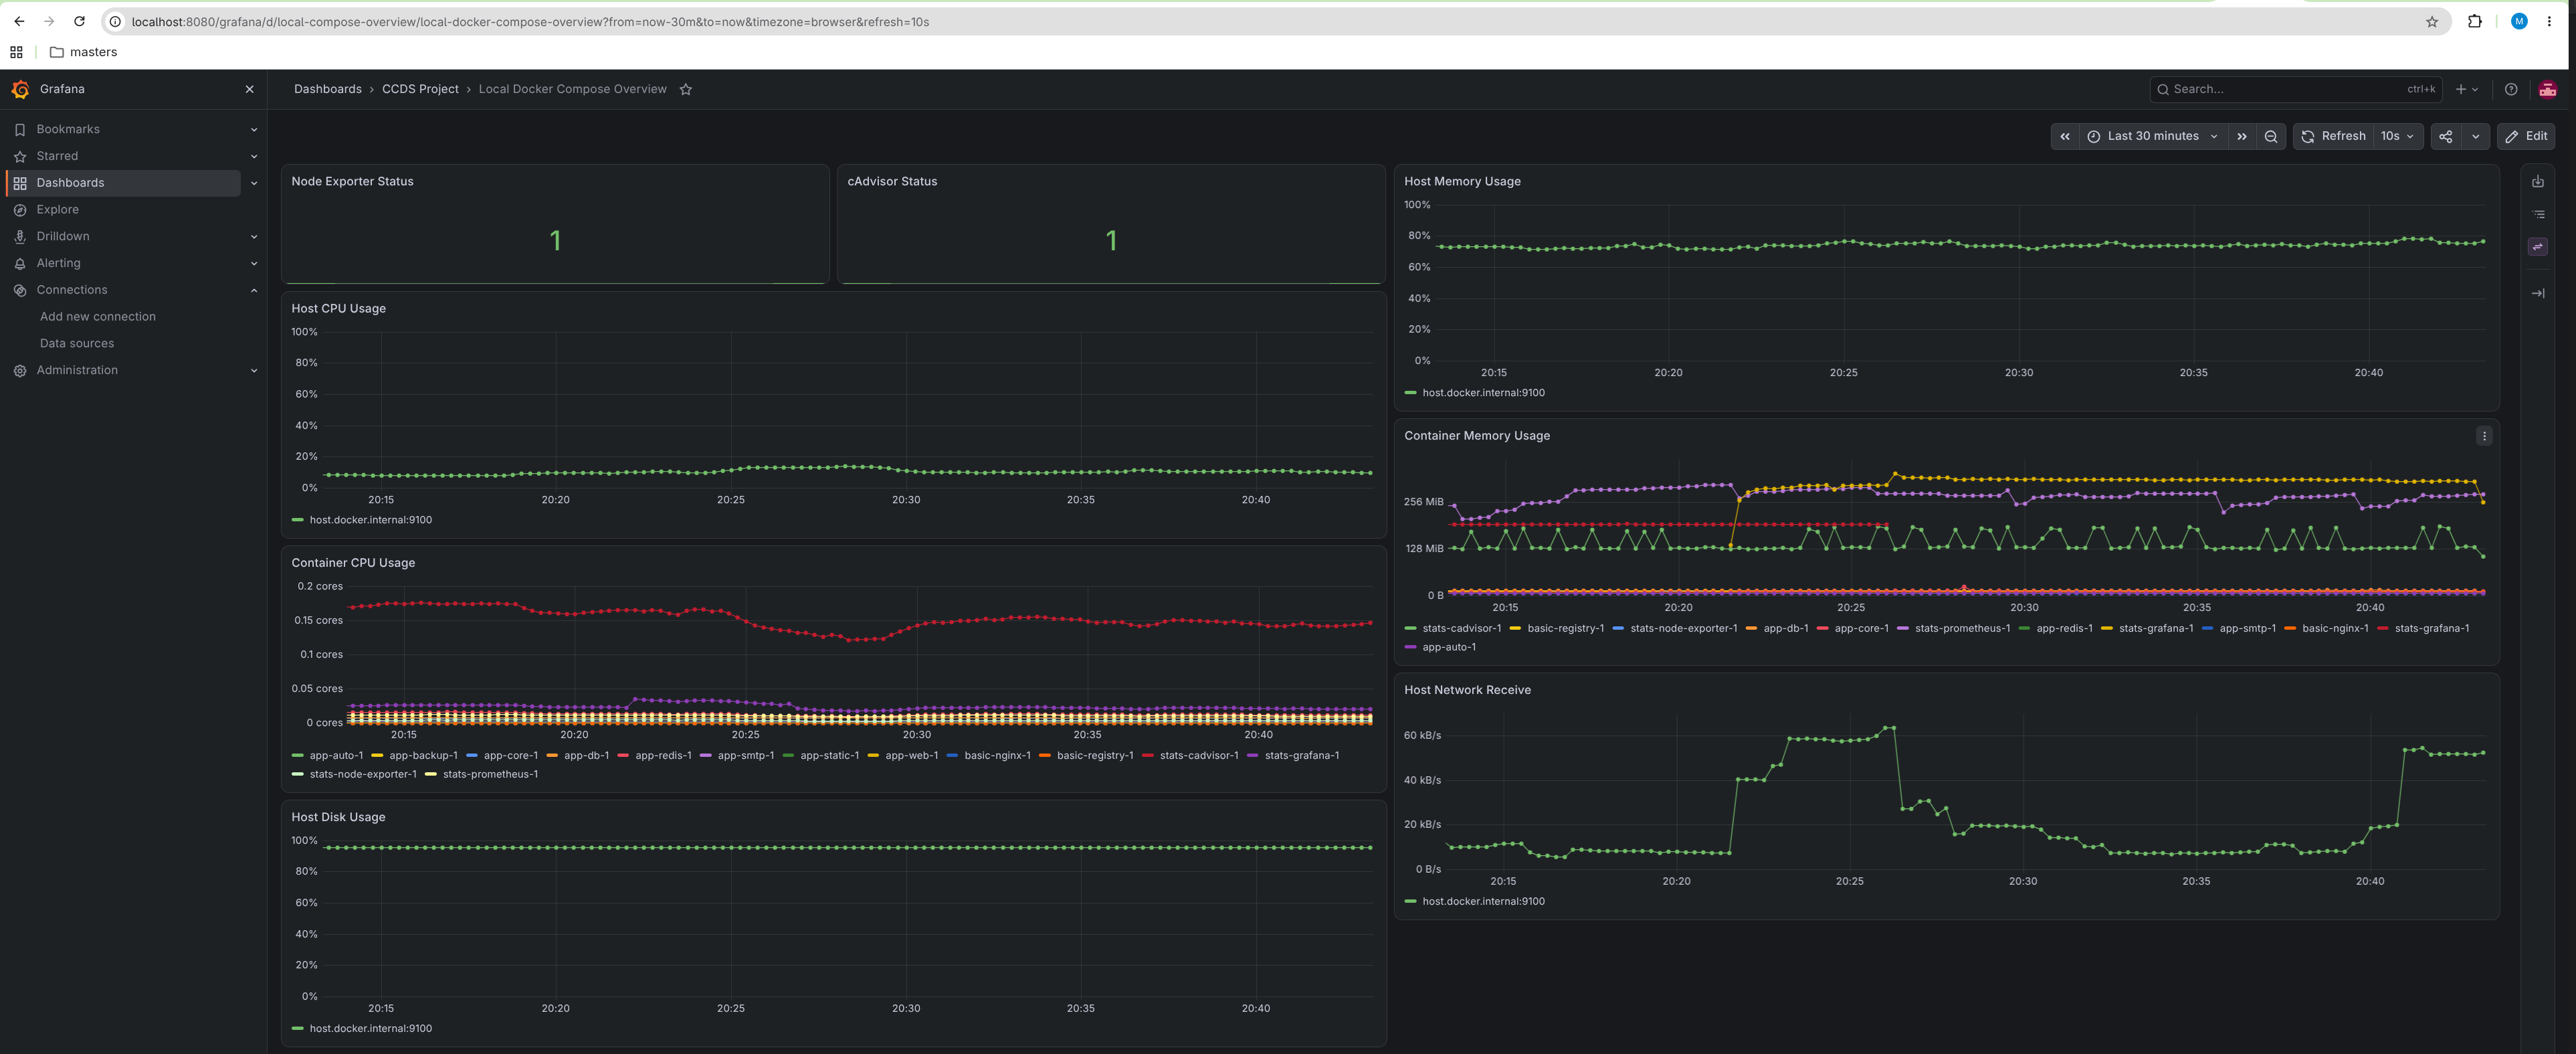
\includegraphics[width=\textwidth]{figures/local-dashboard.png}
\caption{Grafana dashboard for local Compose monitoring.}
\label{fig:local-dashboard}
\end{figure}

\paragraph{On the Swarm.}
Deploy the production stack and inspect the services and logs:
\begin{shell}
sudo docker stack deploy -c stats/production.yml monitoring
sudo docker stack services monitoring
sudo docker service ps monitoring_prometheus
sudo docker service ps monitoring_grafana
sudo docker service logs monitoring_prometheus
\end{shell}

Check that the services have the expected replica counts. In
Prometheus, verify that the Node Exporter and cAdvisor targets are
healthy and that metrics are being collected from the Swarm nodes.
Then open Grafana through the configured nginx URL and confirm that
the provisioned dashboard displays current data.

The production dashboard is shown in \Cref{fig:production-dashboard}.
\begin{figure}[htbp]
\centering
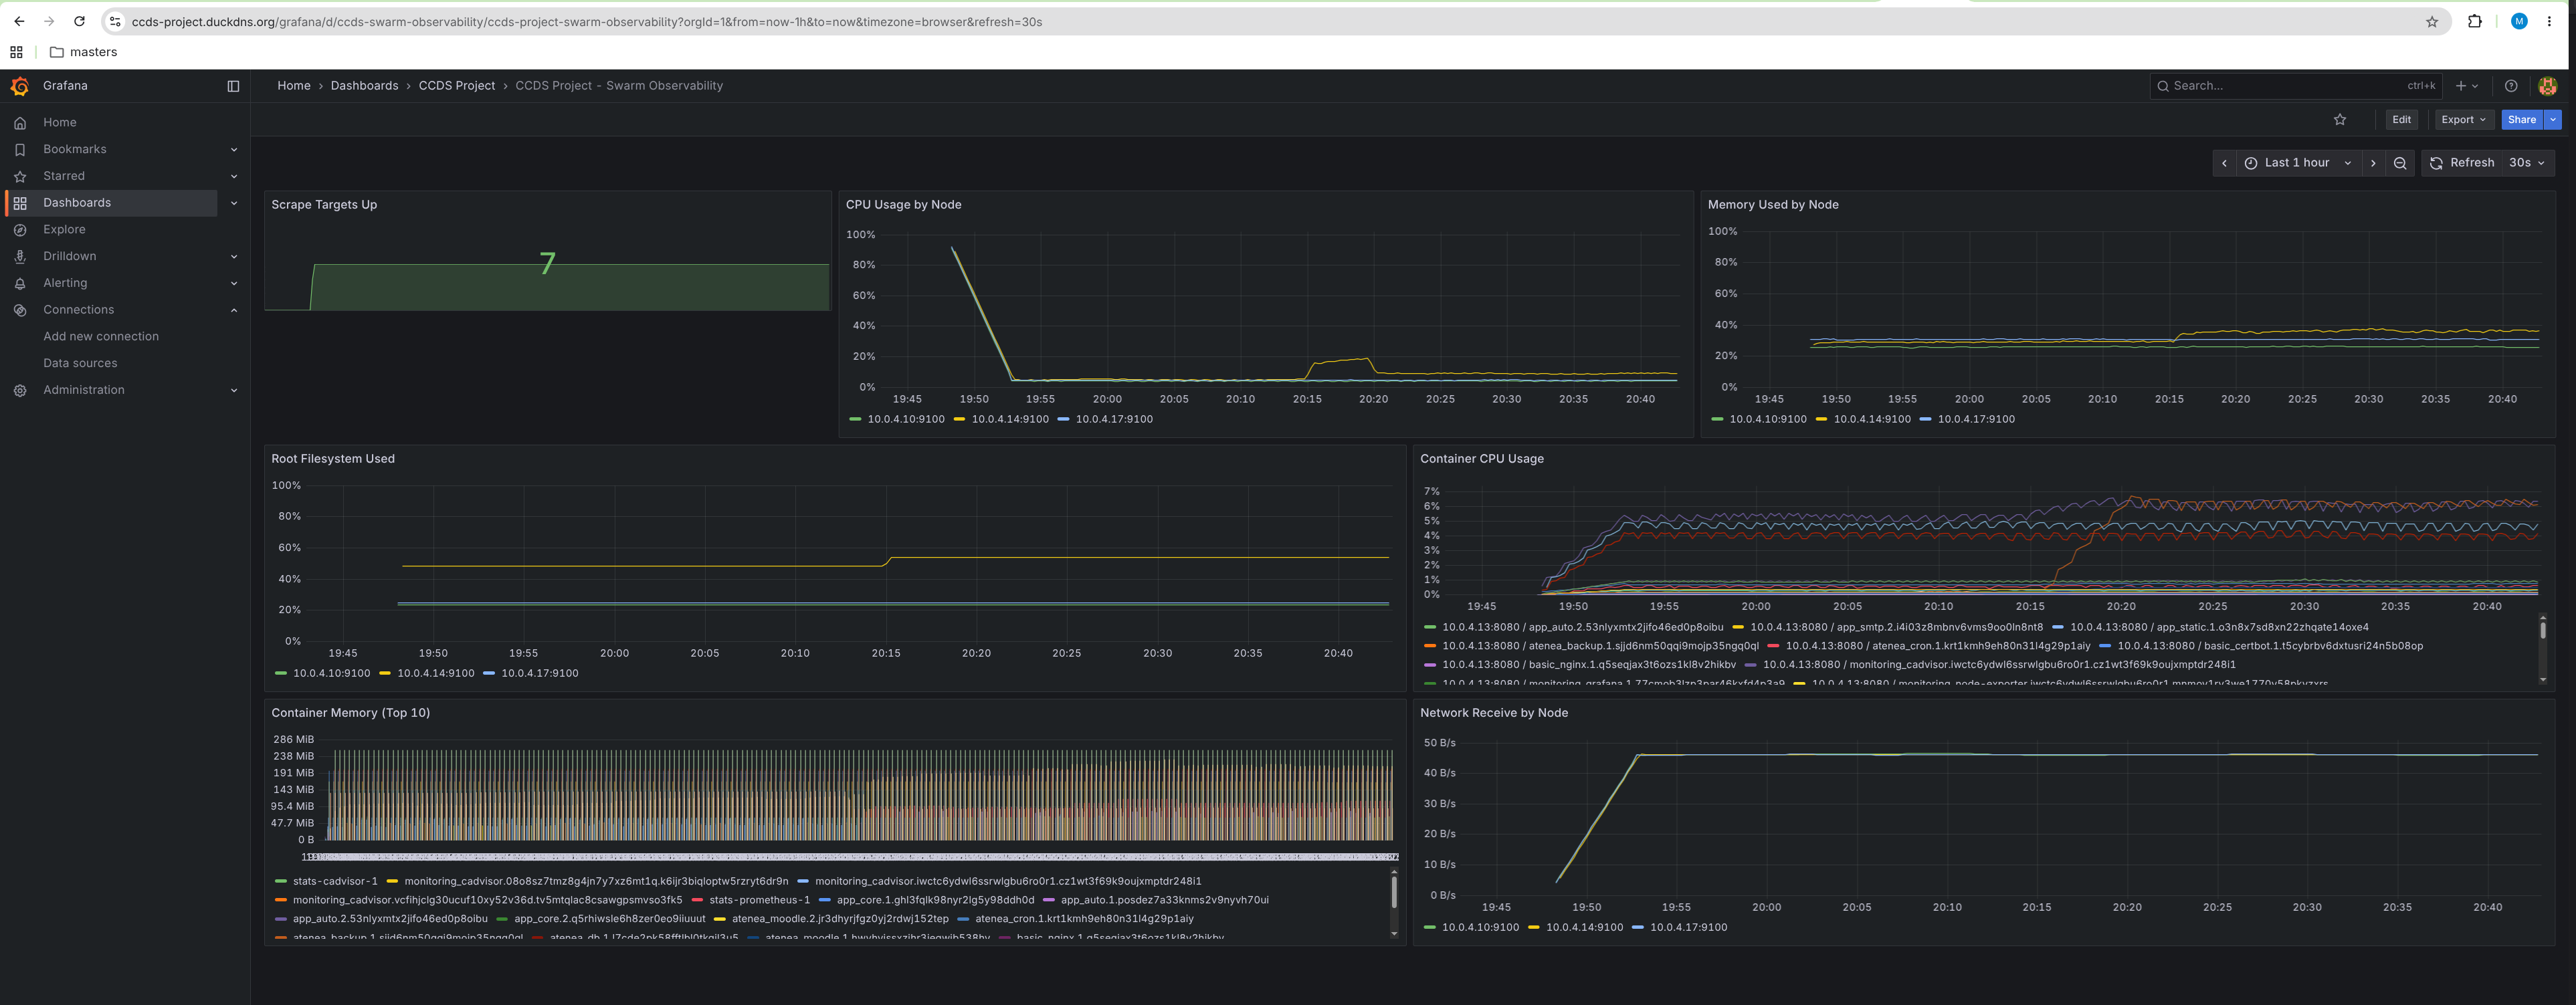
\includegraphics[width=\textwidth]{figures/production-dashboard.png}
\caption{Grafana dashboard for Swarm production monitoring.}
\label{fig:production-dashboard}
\end{figure}

Finally, verify that monitoring continues to work after restarting
a service and that the dashboards recover when Prometheus becomes
available again. Record the actual results of these tests.

%% Owner: Víctor Martín Castilla, with each stack owner for their rows
\section{Data and backups}
\label{sec:data}

The course defines data by what is lost if it disappears
\parencite{llusa2026volumes}. Critical data must be backed up. Volatile
data can be recomputed, even if slowly. Configuration and code are not
data: they belong in images, environment variables, configs or secrets,
and they live in git. \Cref{tab:data} classifies everything the
infrastructure stores with that rule.

\begin{table}[htbp]
  \centering
  \caption{What the infrastructure stores, where, and how it is protected.}
  \label{tab:data}
  \small
  \begin{tabular}{llll}
    \toprule
    Data                  & Where                         & Class         & Protection \\
    \midrule
    App database          & PostgreSQL, database node   & critical      & dump, off-site copy \\
    Moodle database       & MariaDB, database node      & critical      & dump, off-site copy \\
    Moodle files          & NFS share          & critical      & copy, off-site copy \\
    Registry images       & NFS share          & recomputable  & rebuilt from git \\
    TLS certificates      & NFS share          & recomputable  & reissued by certbot \\
    Prometheus metrics    & local volume & volatile      & loss accepted \\
    Redis cache           & memory                        & volatile      & discarded \\
    Dashboards, settings  & git                           & configuration & provisioned from files \\
    Container logs        & stdout, rotated               & operational   & \todo{decide} \\
    \bottomrule
  \end{tabular}
\end{table}

Backups follow one path. Each database dump job writes compressed dumps
to \texttt{/srv/nfs/backups/<stack>/} on the NFS server, which must be a
different machine from the database node. A nightly job in
the basic stack copies that folder to storage outside Azure, so neither
a lost node nor a lost region takes the backups with it. The course
stresses that backups only count once a restore has been tested
\parencite{llusa2026hadr}.

\todo{off-site target, schedule and retention; restore test with
timings for each database.}

%% Owner: Víctor Martín Castilla
\section{High availability and disaster recovery}
\label{sec:hadr}

High availability recovers from minor outages automatically; disaster
recovery restores service after a major one, by hand and from backups
\parencite{schmidt2006ha,llusa2026hadr}.

\subsection{High availability}
\label{sec:hadr-ha}

\begin{itemize}
  \item Three managers keep the Swarm manageable when one node fails
        (\cref{sec:infra-three}).
  \item Stateless services run at least two replicas spread over the
        nodes. Swarm restarts failed tasks elsewhere and the routing mesh
        balances requests between replicas.
  \item Health checks let Swarm replace containers that are running but
        no longer working \parencite{llusa2026production}.
  \item Rolling updates replace one replica at a time and roll back
        automatically when the new version fails.
\end{itemize}

\todo{List the single points of failure of the cluster the team uses,
such as the public entry, the NFS server, the database node and the
Azure region, and measure what happens when each node is stopped.}

\subsection{Disaster recovery}
\label{sec:hadr-dr}

\todo{choose the service category with the team and justify it. As a
starting point, Schmidt's ``business-important'' category allows a
recovery time objective (RTO) of three days and a recovery point
objective (RPO) of one day \parencite{schmidt2006ha}, which daily dumps
satisfy. Document the recovery procedure from zero and its measured
duration.}

%% Owner: Víctor Martín Castilla
\section{Deployment}
\label{sec:deployment}

Every deploy runs on \texttt{swarm-manager-1}, from a checkout of the
repository, because it is the only node reachable by SSH and it keeps the
secret files. Each stack's README holds the details. This section gives
the order and the exact commands.

Two things are prepared once. The shared network, with
\texttt{docker network create --driver overlay proxy}, and each stack's
secret files, which git ignores because the repository is public: the
registry's password file for basic; the database password, feed token
and SMTP settings for app; and the database, root and admin passwords
for atenea. Then every deploy follows the same steps, basic first,
because the other stacks reach the internet through its nginx:

\begin{shell}
ssh azureuser@ccds-project.duckdns.org
cd ccds-project && git pull
sudo docker login ccds-project.duckdns.org

# basic: build and push its two images, then deploy
sudo docker build -t ccds-project.duckdns.org/nginx-proxy:1.6 basic/nginx
sudo docker push ccds-project.duckdns.org/nginx-proxy:1.6
sudo docker build -t ccds-project.duckdns.org/certbot:1.2 basic/certbot
sudo docker push ccds-project.duckdns.org/certbot:1.2
sudo docker stack deploy --with-registry-auth -c basic/compose.yml basic

# app and atenea: each stack has a build script
sudo app/build.sh
sudo docker stack deploy --with-registry-auth -c app/production.yml app
sudo atenea/build.sh
sudo docker stack deploy --with-registry-auth -c atenea/production.yml atenea

# every service must show all its replicas, such as 2/2
sudo docker stack services basic
sudo docker stack services app
sudo docker stack services atenea
\end{shell}

The \texttt{--with-registry-auth} flag hands the login to every node, so
the nodes can pull the team's images. Two steps need patience. When
certbot adds a subdomain to the certificate, nginx keeps serving the old
certificate until it restarts, with
\texttt{docker service update --force basic\_nginx}. On the first atenea
deploy, the web replicas start only after \texttt{cron} has installed
Moodle, which takes a few minutes. \Cref{tab:versions} lists the image
versions deployed.

\begin{table}[htbp]
  \centering
  \caption{Image versions deployed. The team's images live in its
    registry, the others come from Docker Hub.}
  \label{tab:versions}
  \small
  \begin{tabular}{l>{\raggedright\arraybackslash}p{105mm}}
    \toprule
    Stack  & Images \\
    \midrule
    basic  & \texttt{nginx-proxy:1.6}, \texttt{certbot:1.2}, \texttt{registry:3.1.2} \\
    app    & \texttt{app-core}, \texttt{app-static}, \texttt{app-db}, \texttt{app-smtp},
             \texttt{app-backup} and \texttt{app-auto}, all \texttt{1.2};
             \texttt{redis:8.2-alpine} \\
    atenea & \texttt{atenea-moodle:1.0}, \texttt{atenea-backup:1.0}, \texttt{mariadb:11.4} \\
    stats  & \todo{Mikael: the images of the stats stack.} \\
    \bottomrule
  \end{tabular}
\end{table}

%% Owner: Víctor Martín Castilla
\section{Team organisation}
\label{sec:team}

The team has three members, and each owns whole stacks
(\cref{tab:team}). Mikael built the Azure cluster and the basic stack
first. The remaining stacks were then split so that nobody waits for
anybody else.

\begin{table}[htbp]
  \centering
  \caption{Ownership of the work.}
  \label{tab:team}
  \begin{tabular}{ll}
    \toprule
    Member                  & Owns \\
    \midrule
    Mikael Rodriguez        & Azure cluster, basic stack, stats stack \\
    Bernat Ventura          & app stack \\
    Víctor Martín Castilla  & security review and fixes, atenea stack, report \\
    \bottomrule
  \end{tabular}
\end{table}

All the work lives in one shared GitHub repository, with one folder per
stack. Changes reach the main branch through pull requests, so another
member reviews each one before it is deployed. Laptops are only the
development environment: each member runs their stack locally with its
local Compose file, and the production file is what gets deployed to
the Swarm.
\todo{describe the conventions the team agreed on, such as names,
networks and secrets.}

%% Owner: Víctor Martín Castilla
\section{Conclusions}
\label{sec:conclusions}

The basic and app stacks run on a three-node Swarm on Azure, behind one
public entry with HTTPS, and the atenea stack is built, tested on a
laptop and ready to deploy. \todo{Mikael: one sentence on the stats
stack.} Data outlives containers: the app's database moved between nodes
with its data intact, and Moodle came back from a backup in
\qty{21}{\second}. Secrets never reach the public repository, stateless
services update one replica at a time with automatic rollback, and the
internet reaches only ports 22, 80 and 443 of one node.

Several things do not work as they should yet:
\begin{itemize}
  \item The registry login is merged but not active. On 19 October the
        registry still answered without a password, so anyone could push
        an image under a tag the cluster runs.
  \item The backups share a disk with the data they protect
        (\cref{sec:data}).
  \item nginx runs once, pinned to the node that keeps its certificates,
        and it does not reload them after a renewal.
  \item All members share one administrator account.
  \item The logs of most containers never rotate.
\end{itemize}

Three lessons stand out. First, the details of shared storage decide
what containers can do: root squashing, a sensible default, broke the
registry, and turning it off made every container that mounts the share
root over all of it. Second, Swarm has no start order, so a stack must
coordinate its own start, as Moodle's install marker does. Third, a
backup only counts after a timed restore: Moodle's first drill seemed to
fail, and only the event log showed why.

The obvious next step is an off-site copy of the backup folders, which
would keep the recovery objectives even if \texttt{swarm-manager-1} were
lost. After it come the registry login, the certificates on the shared
disk so nginx can scale, and personal accounts for each member.


%% ---------------------------------------------------------------- back matter
\printbibliography[heading=bibintoc]

\end{document}
